\documentclass[a4paper, 11pt]{article}
\usepackage{a4wide}
\usepackage {amsmath}
\usepackage{amsfonts}
\usepackage {graphicx}
\usepackage[utf8]{inputenc} 
\usepackage[francais]{babel}
\usepackage{fancyhdr}
\usepackage{setspace}
\usepackage{fancyhdr}
\usepackage{lastpage}
\usepackage{extramarks}
\usepackage{chngpage}
\usepackage{soul}
\usepackage[usenames,dvipsnames]{color}
\usepackage{graphicx,float,wrapfig}
\usepackage{ifthen}
\usepackage{listings}
\usepackage{courier}
\usepackage{esint}
\usepackage{stmaryrd}
\usepackage{enumitem}
\usepackage{wrapfig}   % Pour utiliser l'environnement wrapfigure
\usepackage{booktabs} % Pour des lignes horizontales améliorées
\usepackage{algorithmicx} 
\usepackage{algpseudocode} 
\usepackage{multicol}

\lhead{} 
\chead{} 
\rhead{\bfseries Méthode projective de Galerkin} 
\lfoot{JC Toussaint}
%\cfoot{} 
%\rfoot{\thepage}

% This is the color used for MATLAB comments below
\definecolor{MyDarkGreen}{rgb}{0.0,0.4,0.0}

% For faster processing, load Matlab syntax for listings
\lstloadlanguages{Matlab}%
\lstset{language=Matlab,                        % Use MATLAB
        frame=single,                           % Single frame around code
        basicstyle=\small\ttfamily,             % Use small true type font
        keywordstyle=[1]\color{Blue}\bf,        % MATLAB functions bold and blue
        keywordstyle=[2]\color{Purple},         % MATLAB function arguments purple
        keywordstyle=[3]\color{Blue}\underbar,  % User functions underlined and blue
        identifierstyle=,                       % Nothing special about identifiers
                                                % Comments small dark green courier
        commentstyle=\usefont{T1}{pcr}{m}{sl}\color{MyDarkGreen}\small,
        stringstyle=\color{Purple},             % Strings are purple
        showstringspaces=false,                 % Don't put marks in string spaces
        tabsize=5,                              % 5 spaces per tab
        %
        %%% Put standard MATLAB functions not included in the default
        %%% language here
        morekeywords={xlim,ylim,var,alpha,factorial,poissrnd,normpdf,normcdf},
        %
        %%% Put MATLAB function parameters here
        morekeywords=[2]{on, off, interp},
        %
        %%% Put user defined functions here
        morekeywords=[3]{FindESS, homework_example},
        %
        morecomment=[l][\color{Blue}]{...},     % Line continuation (...) like blue comment
        numbers=left,                           % Line numbers on left
        firstnumber=1,                          % Line numbers start with line 1
        numberstyle=\tiny\color{Blue},          % Line numbers are blue
        stepnumber=5                            % Line numbers go in steps of 5
        }

% Includes a MATLAB script.
% The first parameter is the label, which also is the name of the script
%   without the .m.
% The second parameter is the optional caption.
\newcommand{\matlabscript}[2]
  {\begin{itemize}\item[]\lstinputlisting[caption=#2,label=#1]{#1.m}\end{itemize}}

\pagestyle{fancy}

\begin{document}

\title{Formulation éléments finis : application à l’équation de l’électrocinétique}

%\author{Jean-Christophe Toussaint\\
%  Phelma\\
%\texttt{jean-christophe@phelma.grenoble-inp.fr}
%}
%\vspace{-2cm}
\date{\today}
 
\maketitle

On résume ici les notions à maîtriser permettant d'écrire une formulation intégrale faible
associée à une équation de type laplacienne, de la discrétiser sur un maillage éléments finis,
de la résoudre en appliquant des conditions de type Neumann ou Dirichlet.

\begin{wrapfigure}{r}{0.3\textwidth}
  \centering
  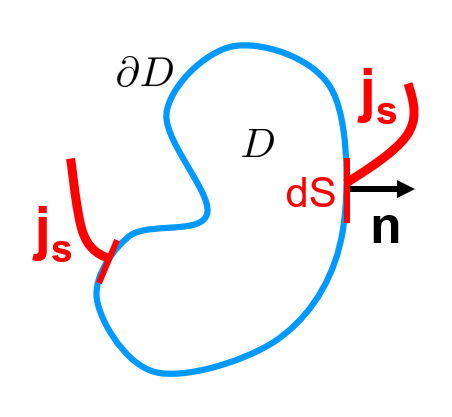
\includegraphics[scale=0.4]{domaine_calcul.png}
\caption{Domaine de calcul}
\end{wrapfigure}


\section{forme forte : }

L’équation locale de l’électrocinétique appelée  ''forme forte'', s’écrit :

%\begin{wrapfigure}{r}{3cm}
%  \centering
%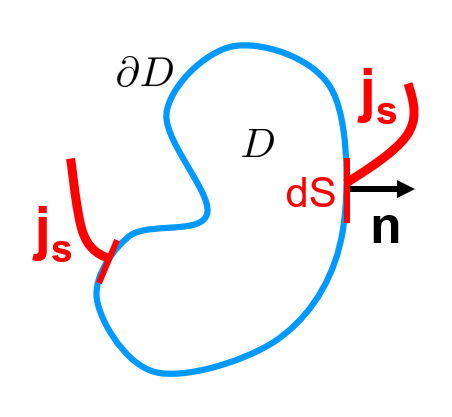
\includegraphics[scale=0.5]{domaine_calcul.png}
%\caption{Domaine de calcul}
%\label{domaine}
%\end{wrapfigure}

\begin{equation}
div\left( {\bf{j}} \right) = 0\quad  \Leftrightarrow \quad div\left( { - \sigma \;\nabla V} \right) = 0
\label{edp}
\end{equation}

avec des conditions aux limites de flux imposées en surface:
\begin{equation}
{\bf{j}} \cdot {\bf{n}} =  - \sigma \;\left( {\nabla V} \right) \cdot {\bf{n}} = j_n^s
\end{equation}



On ne tient pas compte pour l'instant des conditions de type dirichlet qui nécessiteront un traitement
particulier.

\section{forme faible :}

On projette l'équation \eqref{edp} sur des fonctions tests $\omega \in H_1$, espace
fonctionnel dans lequel $\omega$ et ses dérivées au sens des distributions, sont
de carré sommable. La formulation faible (ou forme faible) s’écrit :

\begin{equation}
\int\limits_D {{d^3}r\;{\omega}\;} \left( {div\;{\bf{j}}} \right) = 0\quad  \Leftrightarrow \quad \int\limits_D {{d^3}r\;{\omega}\;} div\left( { - \sigma \;\nabla V} \right) = 0
\end{equation}

Pour faire apparaître les conditions aux limites, une intégration par partie est nécessaire en utilisant l’identité de Green :

\begin{equation}
\int\limits_D {{d^3}r\;\sigma \;\nabla {\omega} \cdot \nabla V\;}  + \oiint\limits_{\partial D} 
 {dS\;} {\omega}\;{\bf{j}} \cdot {\bf{n}} = 0
\end{equation}

En tenant compte des conditions aux limites de flux imposées en surface (sur $\partial D$), la forme faible devient :
\begin{equation}
\int\limits_D {{d^3}r\;\sigma \;\nabla {\omega} \cdot \nabla V\;}  =  - \oiint\limits_{\partial D} 
 {dS\;} {\omega}\;j_n^s
\label{weak}
\end{equation}

\section{formulation éléments finis:}

En 3D, on discrétise le domaine de calcul $D$ en éléments finis de volume (tétraèdres ou hexaèdres) et sa trace 
(surface) $\partial D$ en éléments finis de surface (triangles ou quadrangles). Le maillage 
doit être conforme : i) il est formé d'éléments finis jointifs sans recouvrement entre éléments,
ii) deux éléments jointifs partagent les mêmes noeuds. 

La fonction test $\omega$ est construite par interpolation sur le maillage éléments finis :

$\omega\left( {\bf{r}} \right) = \sum\limits_{i\in e} {{\alpha _i^e}\left( {\bf{r}} \right)\;{\omega_i}} $,
où la somme est restreinte sur la liste des noeuds de l'élément e dans lequel est localisé {\bf{r}}.

L’inconnue V est elle-aussi approximée par son interpolée  :
$V\left( {\bf{r}} \right) = \sum\limits_{j\in e} {{\alpha _j^e}\left( {\bf{r}} \right)\;{V_j}} $.

En utilisant la propriété d'additivité des intégrales et les approximations précédentes,  l'équation $\eqref{weak}$ devient :

\begin{equation}
\sum\limits_{e / {vol}}{} \sum\limits_{(i,j) \in e}  \omega_i \left( {\int\limits_e {{d^3}r\;\sigma \;\nabla {\alpha_i^e} \cdot \nabla {\alpha _j^e}} } \right)\,{V_j}\; =  - \sum\limits_{e / {surf}}{}  \sum\limits_{i \in e}  \omega_i  \iint\limits_{e} 
 {dS\;} {\alpha _i^e}\;j_n^s
\label{dsc_weak1}
\end{equation}
et reste valide pour tout choix du N-uplet $(\omega_1, \omega_2, \ldots, \omega_N) \in \mathbb{R}^N$.

En choisissant d'abord  $(\omega_1=1,\; \omega_2=0, \; \ldots, \; \omega_N=0)$ puis toutes les rotations d'indices, 
l'équation précédente génère un système de $N$ équations linéaires:

\begin{equation}
\sum\limits_{e / {vol}}{} \sum\limits_{j\in e}  \left( {\int\limits_e {{d^3}r\;\sigma \;\nabla {\alpha_i^e} \cdot \nabla {\alpha _j^e}} } \right)\,{V_j}\; =  - \sum\limits_{e / {surf}}{} \iint\limits_{e} 
 {dS\;} {\alpha _i^e}\;j_n^s
\label{dsc_weak}
\end{equation}
où $i \in [1, N]$.

La matrice élémentaire $A_{ij}^e = \int\limits_e {{d^3}r\;\sigma \;\nabla \alpha _i^e \cdot \nabla \alpha _j^e} $ est  aussi rencontrée dans d'autres domaines de la physique où intervient une équation laplacienne. En mécanique de la déformation, on l'appelle matrice de raideur.
Bien que sa taille soit $\text{N} \times \text{N}$, elle ne couple en fait que les NBN nœuds  $\left( {i,j} \right)$ appartenant au même élément $e$. C'est donc une matrice extrêmement creuse.
 Pour stocker ses éléments de manière compacte, on utilise la
table de connectivité qui donne la liste des NBN noeuds constituant l'élément de volume e. 
La matrice $A_{ij}^e$ se transforme alors en une matrice dense $A_{ie\, je}^e$ où  $\left( {ie,je} \right) \in \text{NBN}^2$.

De même, l’intégrale  $B_i^e =  - \sum\limits_{e/surf}^{}  \iint\limits_e {dS\;} \alpha _i^e\;j_n^s$ définit un vecteur élémentaire de dimension N, qui ne comporte que NBN termes non nuls. On la récrit
sous une forme compacte $B_{ie}^e$ où $ie \in \text{NBN}$. Notons qu'ici NBN correspond au nombre de noeuds de l'élément de surface.

L'assemblage est l'opération qui consiste à ajouter les contributions venant des matrices (resp. vecteurs) élémentaires dans une matrice (resp. vecteur) globale. On obtient alors une matrice $A$ de taille 
$\text{N} \times \text{N}$ et un vecteur associé au second membre $B$ de dimension N.

\section{Application à un problème bidimensionnel:}

On suppose que le domaine de calcul s'étend à l'infini selon la direction Oz.
La forme faible devient :
\begin{equation}
\iint\limits_D {dS\;\sigma \;\nabla {\omega} \cdot \nabla V\;}  =  - \oint\limits_{\partial D} 
 {dl\;} {\omega}\;j_n^s
\label{weak2D}
\end{equation}
où $\nabla = e_x\; \partial_x + e_y \; \partial_y$.

On suppose ensuite que le domaine $D$ est discrétisé en éléments finis triangulaires (notés $tri$) et son contour $\partial D$ en segments (notés $seg$). La forme faible discrétisée s'écrit alors, en ne tenant compte que des conditions de type Neumann:

\begin{equation}
\sum\limits_{e / {tri}}{} \sum\limits_{j\in e}  \left( {\iint\limits_e {dS\;\sigma \;\nabla {\alpha_i^e} \cdot \nabla {\alpha _j^e}} } \right)\,{V_j}\; =  - \sum\limits_{e / {seg}}{} \int\limits_{e} 
 {dl\;} {\alpha _i^e}\;j_n^s
\label{dsc_weak2D}
\end{equation}
où $i \in [1, N]$. On rappelle qu'en 2D cartésien :  $\nabla {\alpha_i^e} \cdot \nabla {\alpha _j^e} = 
\partial_x \alpha_i^e \; \partial_x \alpha_j^e + \partial_y \alpha_i^e \; \partial_y \alpha_j^e$.

\subsection{Exercice : assemblage de matrices élémentaires}

On considère le maillage suivant formé de 4 éléments triangulaires :
\begin{figure}[!h]
\centering
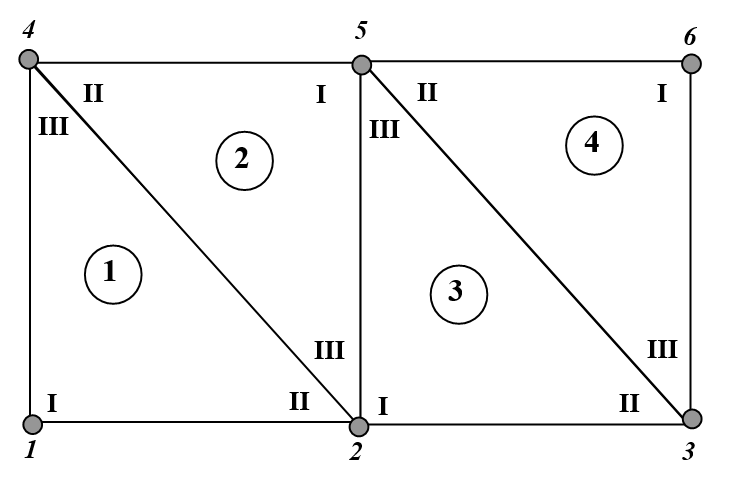
\includegraphics[scale=0.5]{maillage4tri.png}
\caption{maillage formé de 4 triangles}
\label{maillage4tri}
\end{figure}

Sur la figure \ref{maillage4tri}, chaque noeud est identifié avec un numéro unique dans $\llbracket 1, N=6 \rrbracket$ . C'est la numérotation globale.

Les éléments sont numérotés de 1 à 4 et pour chaque élément on fait apparaître la numérotation locale des nœuds (I à III). 

La table de connectivité permettant d’établir le lien entre la numérotation locale et globale est donc la suivante :

\begin{table}
    \centering
    \begin{tabular}{|c||c|c|c|}
        \toprule
        ne & I & II & III \\
        \midrule
        1 & 1 & 2 & 4 \\
        2 & 5 & 4 & 2 \\
        3 & 2 & 3 & 5 \\
        4 & 6 & 5 & 3 \\
        \bottomrule
    \end{tabular}
    \caption{Table de connectivité.}
\end{table}

 
 La matrice élémentaire $A_{ij}^e = \int\limits_e {dS\;\sigma \;\nabla \alpha _i^e \cdot \nabla \alpha _j^e} $ 
 stockée de manière compacte, en utilisant la numérotation locale, 
 a la structure suivante :
 
\begin{equation}
 AE^e = 
 \begin{bmatrix}
    AE_\mathrm{I, I}^e & AE_\mathrm{I, II}^e & AE_\mathrm{I, III}^e \\
    AE_\mathrm{II, I}^e & AE_\mathrm{II, II}^e & AE_\mathrm{III, III}^e \\
    AE_\mathrm{III, I}^e & AE_\mathrm{III, II}^e & AE_\mathrm{III, III}^e \\
\end{bmatrix}
\end{equation}
On ne tient pas compte du fait qu'elle est symétrique.
 
\begin{enumerate}
\item Compte tenu du maillage de la figure \ref{maillage4tri}, quelle est la taille de la matrice globale à résoudre ? 
\item On réalise l’étape d’assemblage de la matrice globale à partir des matrices élémentaires, où sont localisés les éléments non nuls de la matrice globale ? 
\item Ecrire un algorithme permettant de réaliser l’étape d’assemblage d'une matrice élémentaire $AE$
dans une matrice globale $A$ pour un trinagle donné e.
On note {\tt NBN} le nombre de noeuds de l'élément et {\tt ind} la liste des noeuds le constituant.
\end{enumerate}


\subsection{Exercice : assemblage de vecteurs élémentaires}

pour tenir compte du second membre de \eqref{dsc_weak2D}, il est nécessaire
d'ajouter au maillage précédent 6 éléments de type segment sur le contour $\partial D$ (Fig. \ref{maillage4tri6seg}). 
\begin{figure}[!h]
\centering
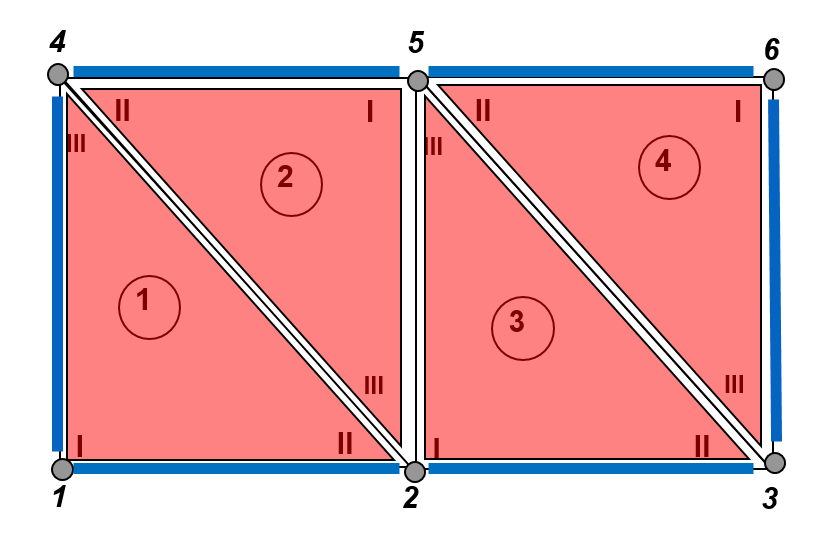
\includegraphics[scale=0.5]{maillage_4tri_6seg.png}
\caption{maillage formé de 4 triangles et de 6 segments}
\label{maillage4tri6seg}
\end{figure}

Le vecteur élémentaire $b_i^e = - \int\limits_{e}  {dl\;} {\alpha _i^e}\;j_n^s$
stocké de manière compacte en utilisant la numérotation locale, 
 a la structure suivante :

\begin{equation}
 BE^e = 
 \begin{bmatrix}
    BE_\mathrm{I}^e \\
    BE_\mathrm{II}^e  \\
\end{bmatrix}
\end{equation}
 
\begin{enumerate}[resume]
\item On réalise l’étape d’assemblage du vecteur global à partir des vecteurs élémentaires, où sont localisés les éléments non nuls du vecteur global ? 
\item Modifier l'algorithme d'assemblage pour qu'il puisse aussi assembler le vecteur élémentaire $BE$
dans un vecteur global $B$ pour un segment donné e.
On note {\tt NBN} le nombre de noeuds de l'élément et {\tt ind} la liste des noeuds le constituant.
\end{enumerate}

\section{Estimation des matrices et vecteurs élémentaires}

Afin d'automatiser les calculs d'intégrales quelle que soit la forme de l'élément considéré, on
introduit la notion d'éléments de référence.
Dans le cas des éléments de forme triangulaire, l'élément de référence est un triangle isocèle rectangle
en 0, de base et de hauteur unité.
Une transformation isoparamètrique $T(u,v)$ permet de déformer élastiquement l'élément de référence
pour lui faire épouser la forme de l'élément réel. Elle utilise les mêmes polynômes de Lagrange $\alpha_{ie}(u,v)$
que l'interpolation de Lagrange d'une grandeur nodale en tout point intérieur de l'élément :

\begin{figure}[!h]
\centering
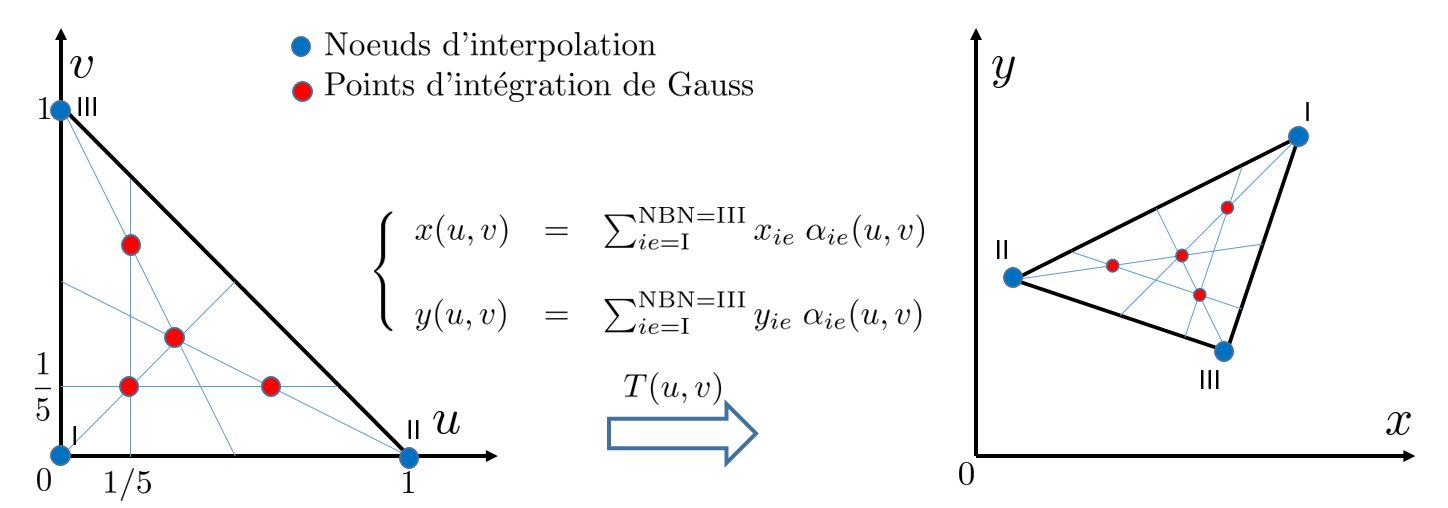
\includegraphics[scale=0.45]{isoparametrique.png}
\caption{Transformation isoparamétrique de l'élément de référence $e_{ref}$
vers l'élément réel $e$}
\label{isopara}
\end{figure}

La matrice élément $A_{ie,je}^e$ peut être estimée par une relation de quadrature de Gauss :
\begin{equation}
A_{ie, je}^e = \int\limits_e {dS\;\sigma \;\nabla \alpha _{ie}^e \cdot \nabla \alpha _{je}^e} = 
\sum_{k=1}^{\text{NPI}} detJ_k \; w_k \; \nabla \alpha _{ie}^e(k)  \cdot \nabla \alpha _{je}^e(k)
\end{equation}

où $w_k$ sont les poids de Gauss dans l'élément de référence $e_{ref}$. Ils
vérifient toujours l'identité $\sum_k w_k=1/2$, surface de $e_{ref}$.

Dans le cas précis où $\text{NPI}=4$ points de Gauss, on a:

\begin{table}
    \centering
    \begin{tabular}{|c|c|c|c|}
        \toprule
        $k$ & $u_k$ & $v_k$ & $w_k$ \\
        \midrule
        1 & 1/3 & 1/3 & $-27/96$ \\
        2 & 1/5 & 1/5 & $+25/96$ \\
        3 & 3/5 & 1/5 & $+25/96$ \\
        4 & 1/5 & 3/5 & $+25/96$ \\
        \bottomrule
    \end{tabular}
    \caption{Points et poids de Gauss.}
\end{table}

La matrice jacobienne est définie par :
\begin{equation}
J(u,v)=
\begin{bmatrix}
    \partial_u x & \partial_v x \\
    \partial_u y & \partial_v y
\end{bmatrix}
=
\begin{bmatrix}
    \sum_{ie=\text{I}}^\text{NBN=III} x_{ie} \; \partial_u  \alpha_{ie}(u,v) &  \sum_{ie=\text{I}}^\text{NBN=III} x_{ie} \; \partial_v  \alpha_{ie}(u,v)  \\
    \sum_{ie=\text{I}}^\text{NBN=III} y_{ie} \; \partial_u  \alpha_{ie}(u,v) &  \sum_{ie=\text{I}}^\text{NBN=III} y_{ie} \; \partial_v  \alpha_{ie}(u,v)  \\
\end{bmatrix}
\end{equation}
où seuls les polynômes de Lagrange dépendent de $(u, v)$.
Comme on connait les positions $(u_k, v_k)$ des points de Gauss dans l'élément de référence, il est facile d'estimer la matrice jacobienne et son déterminant
en ces mêmes points.

La réelle difficulté reste la détermination du gradient $\nabla \alpha_{je}^e= e_x\; \partial_x \alpha_{je}^e+ e_y \; \partial_y \alpha_{je}^e$
où à première vue, interviennent des dérivations dans l'espace réel $(x,y)$ d'une fonction dépendante de $(u,v)$.
Il ne faut pas oublier que $(x,y)$ dépendent de $(u,v)$.

Dans un cadre plus général, la détermination du  gradient $(\partial_x f, \partial_y f)$ d'une fonction $f(x,y)$ où intervient un changement de répère $x(u,v)$ et $y(u,v)$,
nécessite de passer par le calcul de la différentielle $df$. Cela évite de se tromper dans la composition des dérivées partielles.
Pour le physicien, la différentielle $df$ peut être vue comme une différence de potentiel dont la valeur ne dépend du choix de repère
fait par l'observateur.

On peut l'écrire de deux manières différentes :
\begin{equation}
df = \partial_x f \; dx(u,v) + \partial_y f \; dy(u,v) \equiv \partial_u f \; du + \partial_v f \; dv
\end{equation}
En injectant les définitions de $dx = \partial_u x \; du + \partial_v x \; dv$ et $dy = \partial_u y \; du + \partial_v y \; dv$ dans 
l'expression de la différentielle $df$, on obtient le système d'équations suivant :

\begin{equation}
\begin{bmatrix}
    \partial_u x & \partial_u y \\
    \partial_v x & \partial_v y
\end{bmatrix}
\begin{bmatrix}
    \partial_x f \\
    \partial_y f
\end{bmatrix}
=
J^t(u,v)
\begin{bmatrix}
    \partial_x f \\
    \partial_y f
\end{bmatrix}
=
\begin{bmatrix}
    \partial_u f \\
    \partial_v f
\end{bmatrix}
\end{equation}

\noindent
On en déduit que 

\begin{equation}
\begin{bmatrix}
    \partial_x f \\
    \partial_y f
\end{bmatrix}
=
J^{-t}(u,v)
\begin{bmatrix}
    \partial_u f \\
    \partial_v f
\end{bmatrix}
\end{equation}
où $J^{-t}$ est l'inverse de la jabienne transposée.

L'application de la relation précédente pour estimer $\nabla \alpha_{je}^e$ en un point de Gauss $k$ est immédiate :
\begin{equation}
\nabla \alpha_{je}^e(k)=
\begin{bmatrix}
    \partial_x \alpha_{je}^e (x_k, y_k)\\
    \partial_y \alpha_{je}^e (x_k, y_k) 
\end{bmatrix}
=
J^{-t}(u_k, v_k)
\begin{bmatrix}
    \partial_u \alpha_{je}^e(u_k, v_k)  \\
    \partial_v \alpha_{je}^e (u_k, v_k)
\end{bmatrix}.
\end{equation}

L'estimation du vecteur élémentaire $b_{ie}^e = - \int\limits_{e}  {dl\;} {\alpha _{ie}^e}\;j_n^s$ est bien plus simple que le cas précédent.
Il est à noter que le déterminant jacobien n'est dans ce cas que le facteur de dilatation du segment de référence $e_{ref}$
vers le segment réel $e$. On applique la relation de quadrature :
\begin{equation}
b_{ie}^e = - \int\limits_{e}  {dl\;} {\alpha _{ie}^e}\;j_n^s = - \sum_{k=1}^{\text NPI} detJ_k \; w_k \; \alpha_{ie}(k) \; j_n^s .
\end{equation}


\section{Conditions aux limites de Dirichlet :}

Dans la formulation éléments finis proposée ici, les conditions aux limites de flux imposé  apparaissent de manière naturelle en imposant la densité de courant de surface $j_n=j_n ^s$. 
Les conditions de Dirichlet qui consistent à imposer la tension, s'appliquent de manière nodale.

Pour appliquer une condition de Dirichlet à un noeud i du maillage,
la technique la plus simple, consiste à remplacer
la ligne $i$ générée par la formulation \eqref{dsc_weak} par l'équation $V_i=V_i^0$ où
$V_i^0$ désigne la tension appliquée au noeud i.

Cette approche comporte toutefois deux inconvénients : i) le conditionnement de la matrice
est dégradé, ii) la matrice $A$ n'est plus symétrique. Le premier défaut est mineur et peut être corrigé en 
préconditionnant la matrice $A$ par sa partie diagonale. Le second est plus restrictif du point
de vue des méthodes itératives de résolution  car la perte de la symétrie exclut  le gradient conjugué. 
Il faut alors le remplacer par un bigradient conjugué, moins stable et plus gourmand en ressources.

La seconde technique dite de substitution consiste à imposer $\alpha_i=0$ à tout noeud i de Dirichlet. 
Cela revient
à éliminer l'équation générée par \eqref{dsc_weak} associée au noeud $i$.

On forme la liste $l_d$ des noeuds de Dirichlet et la liste complémentaire $l_{dof}$ 
des $N_{dof}$ degrés de liberté où l'on cherche à déterminer le potentiel.

Pour tout noeud $i \in l_{dof}$, l'équation \eqref{dsc_weak} devient :
\begin{eqnarray*}
\sum\limits_{e/vol}^{} {} \sum\limits_{j \in e\; / l_{dof}} {\left( {\int\limits_e {{d^3}r\;\sigma \;\nabla \alpha _i^e \cdot \nabla \alpha _j^e} } \right)} \,{V_j}\; = & -& \sum\limits_{e/surf}^{} {} \iint\limits_e 
 {dS\;} \alpha _i^e\;j_n^s \\
& -& \sum\limits_{e/vol}^{} {} \sum\limits_{j \in e\; / l_{d}} {\left( {\int\limits_e {{d^3}r\;\sigma \;\nabla \alpha _i^e \cdot \nabla \alpha _j^e} } \right)} \,{V_j^d}
\end{eqnarray*}

On prendra garde à la notation : $j \in e /l_{dof}$ signifie que l'on restreint la somme sur tous
les noeuds de l'élément $e$ à ceux contenus dans la liste $l_{dof}$ .

On remarque que la matrice associée au système linéaire est de taille $N_{dof} \times N_{dof}$
et qu'elle reste symétrique après substitution des valeurs de Dirichlet. On peut donc utiliser
la méthode du gradient conjugué comme solveur.

Après résolution, on complète les valeurs du potentiel obtenues aux
$N_{dof}$ degrés de liberté par les $N_d$ valeurs de Dirichlet pour construire
la distribution de potentiel en tout noeud.

\subsection{Algorithme de substitution pour traiter les conditions de Dirichlet}

On présente ici l'algorithme mettant en pratique la seconde technique.
On construit d'abord la matrice globale $A$ et le vecteur global $B$
sans se soucier des conditions de Dirichlet.

On forme ensuite la liste $l_d$ des noeuds de Dirichlet 
où chaque numéro apparait de manière de façon unique ({\it Sous Matlab, la fonction
 {\tt unique}   supprime les doublons dans une liste})
et la liste complémentaire $l_{dof}$ des $N_{dof}$ degrés de liberté.\\

On crée un vecteur vide $V^0$ de dimension $N$, puis
pour chaque noeud $i \in l_d$, on lui affecte la valeur de la tension imposée : $V_i^0 \leftarrow V_i ^d$.
Leur substitution dans le système revient à modifier le vecteur second membre $B \leftarrow B -A V^0$.\\

On forme ensuite une matrice de projection $P$ permettant de passer de l'espace des solutions de
dimension $N$ à celui restreint à $N_{dof}$ degrés de liberté.
Les dimensions de P sont $N_{dof} \times N$ (nombre de lignes $\times$ nombre de colonnes).

On initialise d'abord la matrice $P$ à zéro;
puis en parcourant séquentiellement la liste $l_{dof}$, on impose $P(i, l_{dof}(i))=1$ avec $i \in [1, N_{dof}]$.
On remarque que $P P^t = {\tt Id}(N_{dof})$ .

Une autre façon de construire la matrice $P$ est de l'initialiser avec  la matrice identité ${\tt Id}(N)$
puis de supprimer toutes les lignes correspondant aux noeuds de dirichlet. Cette technique
est bien adaptée à Matlab : si $ld$ est la liste des noeuds de dirichlet sans doublon alors 
$P={\tt Id}(N); \; P(ld, :)=[ \;];$

\begin{figure}[!h]
\centering
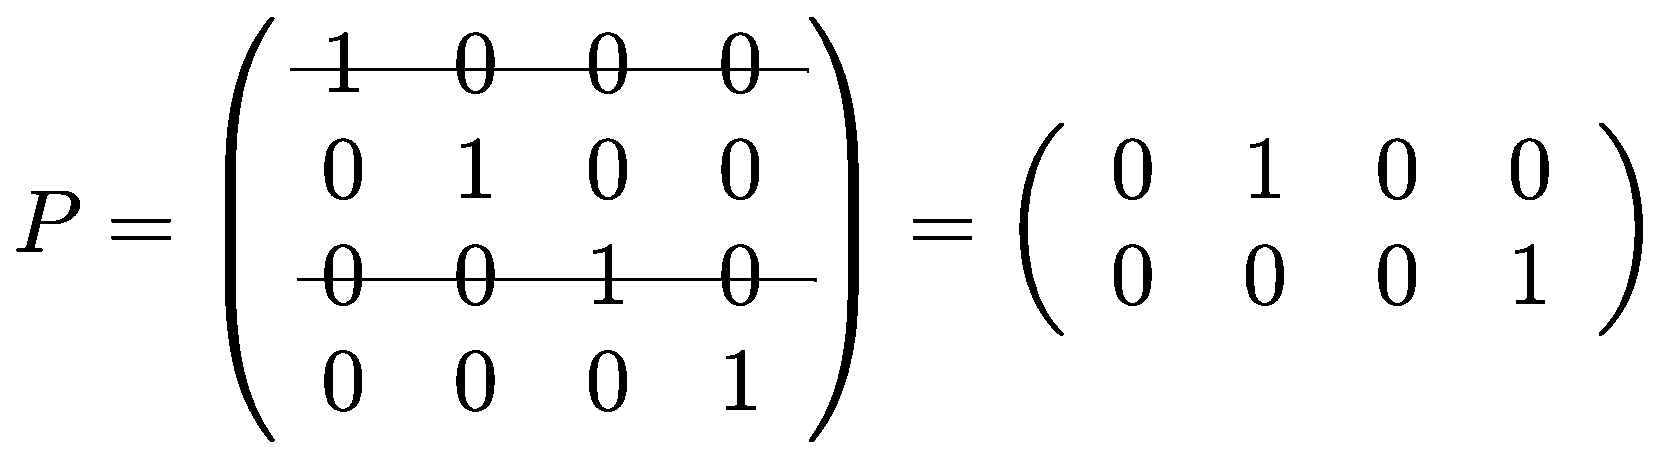
\includegraphics[scale=0.25]{matP.eps}
\caption{exemple de matrice $P$ avec $l_d=\{1, 3\}$}
\label{matP}
\end{figure}

On construit ensuite la matrice projetée $A_p$  de $A$ dans l'espace
solution à $N_ {dof}$ degrés de liberté: $A_p \leftarrow P A P^t$ .
De même pour le vecteur second membre projeté $B_p \leftarrow  P B$.

On donne ci-après un exemple de construction de la matrice projetée $A_p$ à
partir d'une matrice de dimensions 10 $\times$ 10 après application des conditions
de dirichlet aux noeuds  $l_d=\{3, 4, 9\}$:
\begin{figure}[h!]
\centering
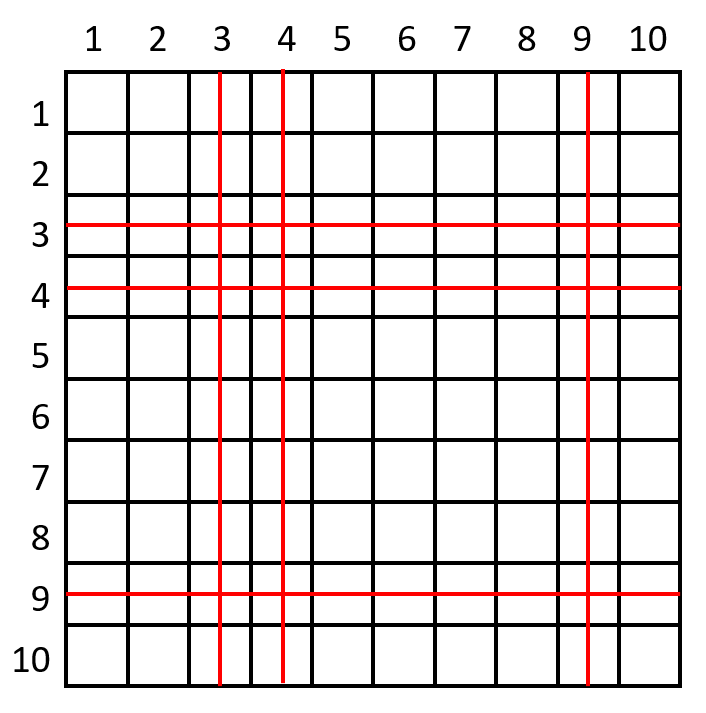
\includegraphics[scale=0.5]{matrice_biffee.png}
\caption{exemple de matrice $A_p$ avec $l_d=\{3, 4, 9\}$}
\label{matP}
\end{figure}

On résout ensuite le systeme d'équations dans  l'espace restreint :
\begin{equation}
A_p V_p = B_p
\end{equation}

On reconstruit finalement la solution dans l'espace à $N$ noeuds en appliquant la
relation:
\begin{equation}
V=P^t \; V_p + V^0
\end{equation}
Elle vérifie automatiquement, $V_i=V_i^d$ en  tout noeud $i$ où la condition de Dirichlet
est appliquée.


\subsection{Exercice : application de la méthode de substitution }


\begin{enumerate}[resume]

\item La matrice globale $A$ est une matrice symétrique définie positive, montrer que 
ses propriétés restent inchangées pour la matrice projetée $A_p$.

\item Mettre en oeuvre la technique de substitution à base de matrices de projection,
pour traiter les conditions de dirichlet, pour l'équation de l'électrocinétique.
Préciser les modifications à apporter  au code éléments finis
fourni initialement.

\item Vérifier que la solution reste inchangée.

%\item Remplacer la méthode de résolution directe par la méthode du gradient, 
%du gradient conjugué voire par sa variante avec un précontionneur diagonal. Utiliser
%soit les routines vues en cours soit celles intégrées dans Matlab.
%Vérifier la cohérence des résultats en utilisant un solveur direct.

%\item Générer une matrice $A$ aléatoire symétrique de taille N $\times$ N, définie positive et
%un vecteur $B$ aléatoire de dimension N.  Imposer en certains noeuds la valeur de l'inconnue.
%Proposer deux implémentations mettant en oeuvre les deux techniques sus-citées pour
%traiter les conditions de Dirichlet.
%
%{\it Indication : pour rendre une matrice définie positive, il suffit que, pour chaque ligne, le terme diagonal soit supérieur à la somme des valeurs absolues des termes non diagonaux }.

%\item Montrer que le solveur gradient conjugué est bien adapté à ce type de système. 
%Vérifier la cohérence des résultats en utilisant un solveur direct.

%\item Reprendre le projet électrocinétique traité précédemment et appliquer-lui,
%l'algorithme de substitution. Mettre en oeuvre un solveur de type gradient conjugué.
%Comparer les résultats obtenus.

\end{enumerate} 


%\section{Algorithme du gradient conjugué avec conditions de dirichlet }
%
%La méthode du gradient conjugué est une méthode itérative pour résoudre un système d'équations linéaires $Ax=b$, où la matrice $A$ de dimension $N \times N$ est symétrique définie positive.
%
%Le principe repose sur la minimisation d'une fonctionnelle quadratique (énergie potentielle) définie dans $\mathbb{R}^N$ :
%$$\mathcal{E}(x) = \frac{1}{2}x^T A x - x^T b$$
%
%On peut démontrer que le minimum $x_\infty$ de cette fonctionnelle correspond exactement à la solution du système linéaire.
%
%En pratique, à partir d'un vecteur initial $x_0 = 0$, la méthode calcule à chaque itération $k$ une nouvelle approximation $x_k$ de la solution en minimisant l'énergie potentielle de manière monotone le long de directions de recherche conjuguées. Cette approche garantit une convergence théorique en au plus $N$ itérations pour un système de dimension $N$.
%
%L'algorithme ci-après est une version adaptée de la méthode du gradient vue en cours,
%dans laquelle est appliquée la stratégie de descente expliquée précédemment.
%Pour éviter que le processus ne s'arrête jamais dans le cas où $b$ est nul, on effectue
%un changement de variable en écrivant  le vecteur inconnu V sous la forme de $V=x+V_d$. 
%Ce qui revient à résoudre $A\; x = b-A\; V_d$.
%Noter que le symbole $\rhd$ désigne le début d'un commentaire.
%
%\algrenewcommand{\algorithmiccomment}[1]{\hskip1em$\triangleright$ #1}
%\begin{algorithmic}[1]
%\Function{GRADIENT\_CONJUGUE}{$A, b, V_d, l_d$}
%\State $b \gets b-A \; V_d$ \Comment{changement $V \rightarrow x$}
%\For {$i \in l_d$}
%    \State $b[i] \gets 0$
%\EndFor
%
%\State $k \gets 0$
%\State $x_0 \gets 0$
%\State $r_0 \gets b-A\; x_0$ \Comment{$r_0(i \in l_d) \equiv 0$}
%\For {$i \in l_d$}
%    \State $r_0[i] \gets 0$
%\EndFor
%\State $p_0 \gets r_0$ \Comment{direction initiale}
%
%\While{$\lVert r_k \rVert > tol \; \lVert b \rVert$}
%    \State $\alpha_k \gets \frac{r_k^t \; r_k}{p_k^t \; A \; p_k}$
%    \State $x_{k+1} \gets x_k + \alpha_k \; p_k$ \Comment{$x_{k+1}(i \in l_d) \equiv 0$}
%    
%    \State $r_{k+1} \gets r_k - \alpha_k \; A \; p_k$
%    \For {$i \in l_d$}
%        \State $r_{k+1}[i] \gets 0$
%    \EndFor
%    
%    \State $\beta_k \gets \frac{r_{k+1}^t \; r_{k+1}}{r_k^t \; r_k}$
%    \State $p_{k+1} \gets r_{k+1} + \beta_k \; p_k$ \Comment{$p_{k+1}(i \in l_d) \equiv 0$}
%    
%    \State $k \gets k+1$
%\EndWhile
%
%\State $x_k \gets x_k+V_d$ \Comment{relèvement par $V_d$}
%\State \Return $x_k$
%\EndFunction
%\end{algorithmic}
%
%
%\begin{enumerate} [resume]
%
% \item Analyser l'algorithme et identifier les lignes critiques qui assurent que
%  les composantes de $x_k$ correspondant aux noeuds de dirichlet restent  nulles à chaque itération.
%  
% \item Proposer une implémentation de cet algorithme sous {\tt Matlab}. 
% On rappelle que l'instruction $x(ld)=0$ met à zéro toutes les composantes du vecteur ligne $x$ dont les indices sont stockés dans la liste $l_d$.
%
%\end{enumerate} 

\end{document}

